\section{Visualization of Time-Oriented Data}
Time is an essential aspect of life; everything contains inherent temporal attributes such as the time when a person was born and the time when an event happens. Long before computers were invented, visualization has been used to represent temporal relationship of data. One of the oldest documented timelines was created by Joseph Priestley in his \emph{Chart of Biography} back in 1765 (\autoref{fig:lr-biography-chart}). It shows the lifespans of two thousand famous names along a horizontal time axis, spanning from 1200 BC to 1800 AD. He uses a horizontal line segment to depict a lifespan, and adds dots to either ends to indicate the uncertainty of the reported values. 

\begin{figure}[!htb]
	\centering
	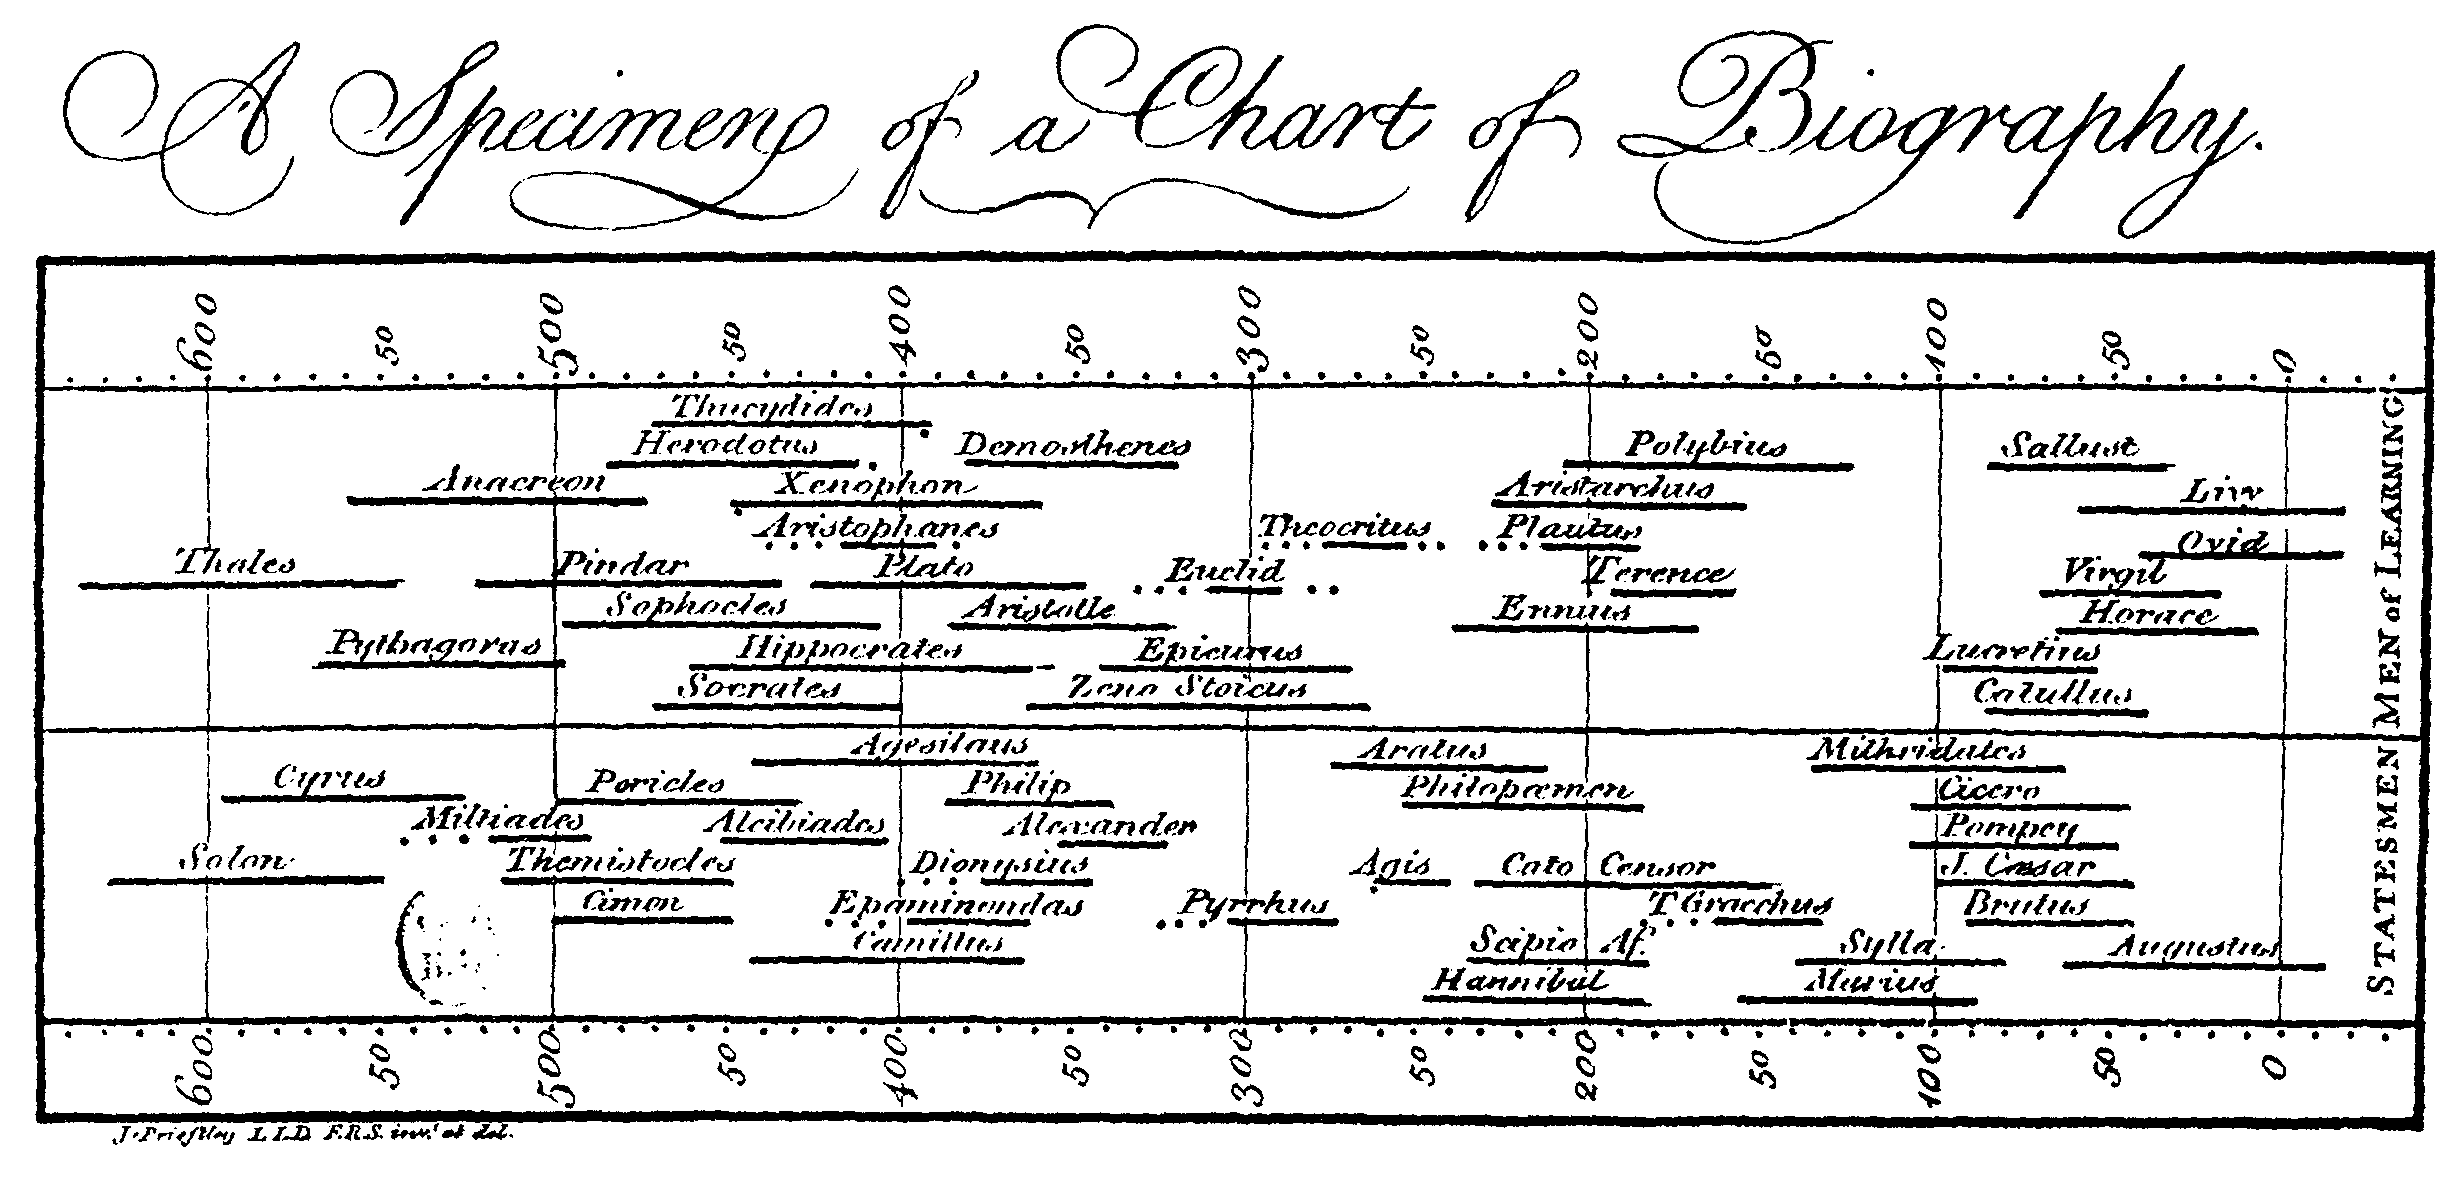
\includegraphics[width=\columnwidth]{biography-chart}
	\caption{Joseph Priestley's chart of biography portraying the lifespans of famous historical
persons. \is{Priestley1765}}
	\label{fig:lr-biography-chart}
\end{figure}

Since then, many visualization techniques have been developed to effectively reveal the temporal relationship of data. The book by Aigner~et~al~\cite{Aigner2011} provides a comprehensive review of this topic. In this section, we focus on different visual mappings of time.

\subsection{Horizontal}
The most common representation of time is mapping it to a horizontal axis as in the aforementioned \emph{Chart of Biography}. Data items are positioned along the axis at when they happen (point-based time) or during which they last (interval-based time). Given a two-dimensional space, the vertical axis is left free for encoding additional information.

\subsubsection{Scaled Vertical Axis}
Time-series data is a sequence of data points collected at uniform intervals such as population of a country every year and stock market value every hour. A time-dependent variable in time-series data is often mapped to the vertical axis. Classic charts such as scatter plot, line chart and bar chart and are all commonly used for this purpose. Scatter plot shows each data point as a dot, with the x-coordinate mapping to the time value and the y-coordinate mapping to the value of the time-dependent variable. Line chart further connects these data points to form a line. Bar chart also shows data points individually like scatter plot, but each point is represented by a bar, with its height corresponding to its value. Line chart is suitable for showing the trend of the series, whereas scatter plot and bar chart are good at emphasizing individual data points. With the advantage of visual alignment, bar chart is more effective than scatter plot at comparison of time-dependent values~\cite{Aigner2011}.

\missingfigure{a figure combining three methods}

Horizon graph~\cite{Reijner2008} is a recent improvement of line chart in time-series data visualization, designed for a more space-efficient representation in order to facilitate comparison of different series; for instance, daily prices for one year of multiple stocks. To make a fair comparison, it shows a derived percentage changes from the earliest data point instead of raw values. Starting from a line chart, the value range is divided into uniform bands, such as 10\% for each band, and color coded using a diverging colormap for positive/negative values with increasing color intensity for greater band values. The colored bands allow more precise value reading. Then, the negative values are mirrored into the positive side, reduced the chart height by half. To save more space, those bands are layered with increasing values, or color intensity, based on the two-tone pseudo coloring technique~\cite{Saito2005}.

\missingfigure{page 158, left figure}

Horizon graph uses space more efficiently than line chart in visualizing time-series data. A study by Heer, Kong and Agrawala~\cite{Heer2009a} investigates their performances in value comparison tasks. The results show that mirroring a chart (flipping negative values) does not have negative effects; it neither slowed completion time nor hurt accuracy. Moreover, for small chart sizes, layered bands are more effective than line chart.

Stacking multiple graphs on top of each other is a suitable approach to visualizing multiple time-dependent variables~\cite{Aigner2011}. ThemeRiver~\cite{Havre2002} can be considered as a ``smooth'' version of stacked graph, designed to show thematic variations over time within a large collection of documents. Each theme is displayed as a colored current flowing through the time, and at any point, the width of the current maps to the strength of the associated theme. The overall river consisting of multiple colored currents provides a good overview of the themes that were important at certain points in time. Byron and Wattenberg discuss considerations of aesthetics and legibility for designing such stacked graphs.

\subsubsection{Non-Scaled Vertical Axis}
The vertical dimension can be used for layout purpose. LifeLines~\cite{Plaisant1996,Plaisant1998} is a visualization system of patient records. It first groups events into different facets such as problems, allergies, diagnosis, and medications, and spatially stack them on top of each other. Within each facet, interval-based events are represented as horizontal bars covering their timespans. Because their timespans can overlap, the layout adjusts the vertical coordinates of the events to avoid intersection. Continuum~\cite{Andre2007} visualizes the lifespans of composers as rectangles, where width represents the temporal information, and height depends on the number of pieces they composed. It also uses vertical position to produce an overlap-free layout.

Data items may have additional relationships besides temporal sequence such as hierarchy and more general pair-wise connections. Gantt chart~\cite{Gantt1913} is a classic visualization commonly used to show planning activities for project management. Each activity is shown as a horizontal bar covering the planning time, and text from the left part of the chart shows activity name. Dependency is a common relationship in planning and can be shown as an arrow. For instance, an arrow pointing from the end of activity $A$ to the beginning of activity $B$ can indicate that $B$ must happen after $A$. Activities often include hierarchy such as tasks and sub-tasks. They can be ordered and arranged with indentation to reflect this structure. Timeline tree~\cite{Burch2008} draws an explicit node-link tree on the left part of the timeline to show the hierarchy.

Another way of using space is through proximity. Storyline visualizations illustrate the dynamic relationships between characters in a movie. The technique was first introduced by Munroe with his hand-drawn charts~\cite{Munroe2009}. The visualization depicts each character as a curved line and each scene a bundle of those character lines. Ideally, all the lines within a scene should be straight and parallel. The line diverges from the bundle if the character leaves the scene, and conversely, the line converges into a bundle if the character joins that scene. Algorithms have been introduced to automate the rendering process including work by Tanahashi and Ma~\cite{Tanahashi2012} and Liu et al.~\cite{Liu2013}. TimeNets applies the idea of using proximity to show relationships in visualizing genealogical data. It uses a curved line to represent a person's lifespan. These lines are located far away if the persons are unrelated. Two lines converge if they marry and diverge if they divorce. Child lines also stay close to their parent lines and connected by dotted vertical lines from the parents to the beginning of their lines to indicate parent-child relationship.

\subsection{Spiral}
spiral: talka bout pattern detection: present/discover;
color-tone
\subsection{Circle}
circle view paage 219 ringmaps?

\subsection{Calendar} [page 177]
finding patterns at different temporal granularities
\subsection{Small Multiples}
p236
\subsection{Animation}
p220